\section{Python Exercise: Multirate Systems}\label{sec:p9}

\begin{figure}[htbp]
	\centering
	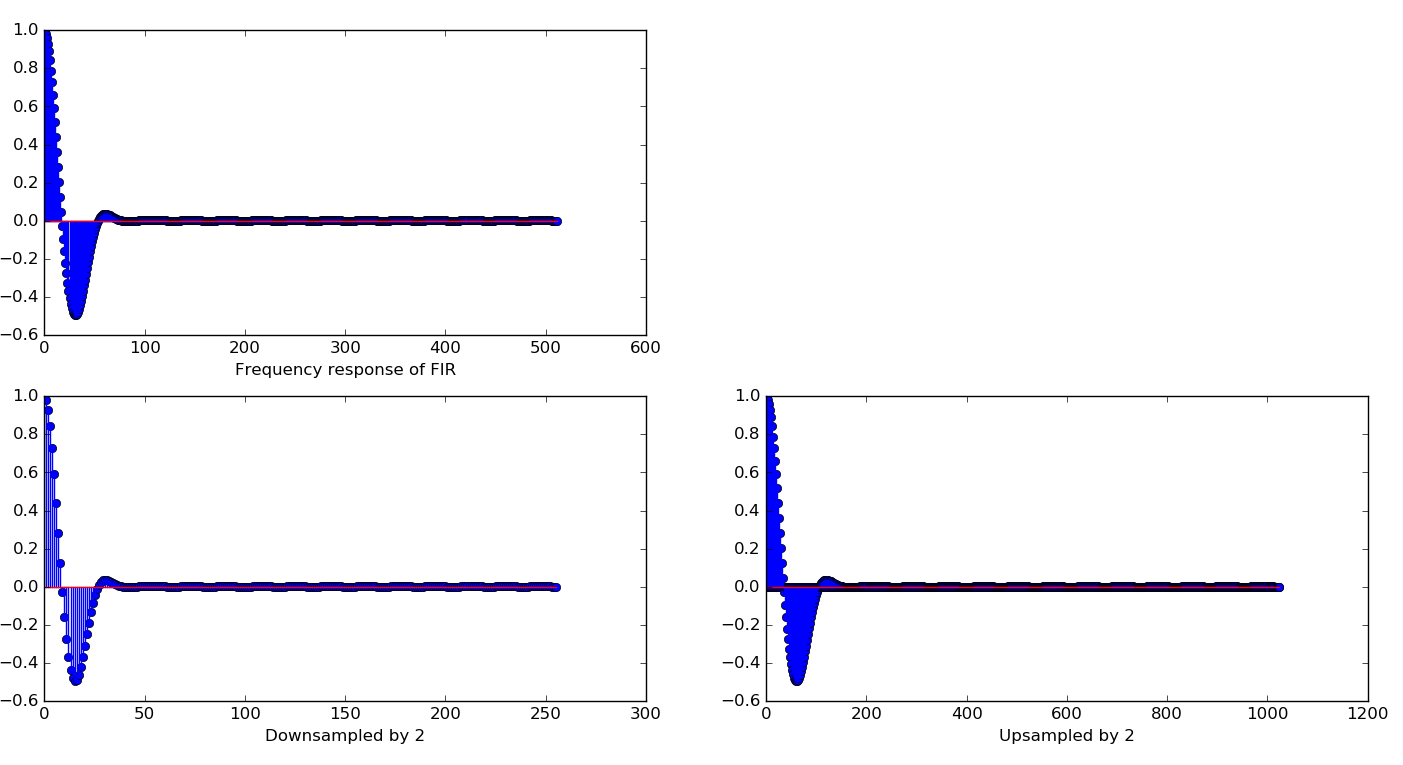
\includegraphics[width=\textwidth]{images/p9-1}
	\caption{An output of generated FIR filter (frequency response).}
	\label{fig:p9-1}
\end{figure}

\begin{figure}[htbp]
	\centering
	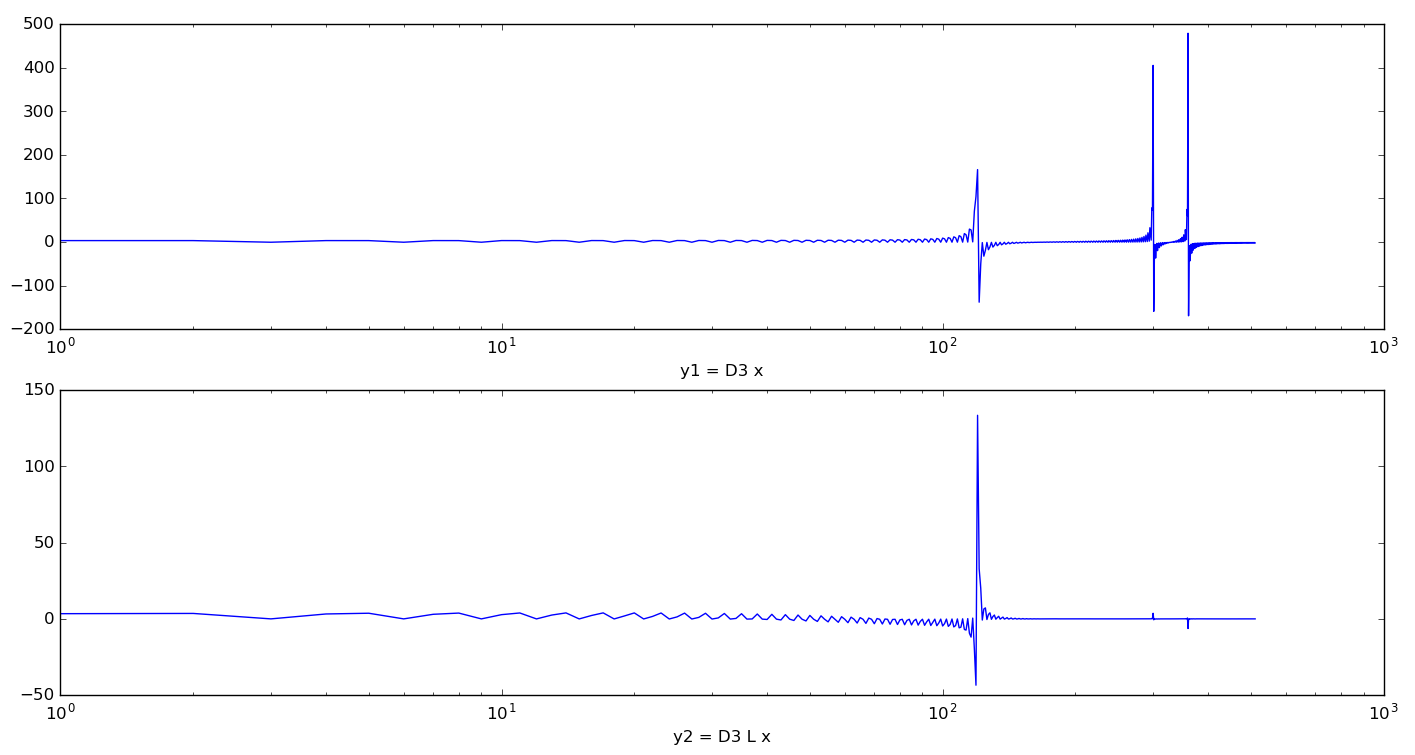
\includegraphics[width=\textwidth]{images/p9-2}
	\caption{An output of $y_1 = D_3 x$ (top) and $y_2 = D_3 L x$ (bottom) (frequency response, in log-scale).}
	\label{fig:p9-2}
\end{figure}

Figure \ref{fig:p9-1} shows the frequency response of FIR lowpass filter (with sample rate of 100). Although the plots look similar due to scaling, the number of samples differs, i.e. downsampled version has half the amount and upsampled version has twice the amount of samples as the original one.

Figure \ref{fig:p9-2}  shows the frequency response of $y_1$ and $y_2$ in log-scale. It is obvious that $y_1$ suffers the aliasing effects (2 spikes towards the end) while that effect on $y_2$ is not significant.